\mainsection{\the\numexpr \thechapter + 1 \relax}{Les boucles}{dd/mm/yyyy}

\vspace{-0.8cm}

\section{Introduction}
En programmation, on appelle boucle un système d’instructions qui permet de répéter un certain nombre de fois (voire indéfiniment) toute une série d’opérations. En Python, comme dans la plupart des langages de programmation il existe deux type de boucle :
\begin{itemize}
	\item La boucle « Pour » (mot-clé \lstinline{for} en Python) qui répète un bloc d’instructions un certain nombre de fois ; Nous découvririons cette boucle en détail dans un prochain cours.
	\item La boucle « tant que » (mot-clé \lstinline{while} en Python) qui exécute un bloc d’instructions tant qu’une condition est vérifée. Dès que la condition devient fausse, elle passe aux instructions qui suivent le bloc :
\end{itemize}



\section{La boucle \textsf{while}}

\begin{mydefinition} La boucle \lstinline{while} permet de répéter un bloc d'instructions tant qu'une condition n'est pas remplie. En python, elle est introduite par le mot-clé \lstinline{while} suivi d'une condition terminé par le symbole ":" 
\end{mydefinition}

\begin{figure}[h]
	\centering
	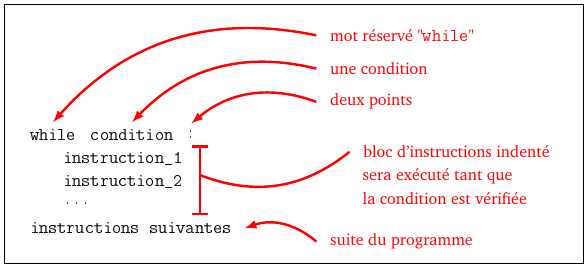
\includegraphics[scale=1]{Images/boucles/while-loop}
	\caption{Figure tirée du \textit{livre Python} au Lycée de Arnaud Bodin.}
	% Source :  https://openclassrooms.com/fr/courses/7168871-apprenez-les-bases-du-langage-python/7296286-repetez-des-taches-facilement-a-l-aide-de-boucles
	%TODO : make smtg similar in latex 
\end{figure}

\newpage

\begin{myexamples}
	\itemb{Compte à rebours des nombres entre 10 et 0:}\\
	\begin{multicols}{2}
		Le programme suivant  
		\begin{lstlisting}
			
		\end{lstlisting}
	\end{multicols}	
	\item Calculer les premières puissances de 2
\end{myexamples}




\subsection{La boucle \textsf{for}}

Si la boucle |while| est la plus modulable, il existe une boucle plus souvent utilisée car plus pratique dans certains cas : itérer un nombre précis de fois, ou parcourir un tableau, etc. C'est la boucle |for|.


\begin{mydefinition} En python, la boucle |for| permet de répéter un bloc d'instructions pour chaque élément d'un container (tableau, chaîne de caractères, etc.). Elle est introduite par le mot-clé |for| suivi d'un nom de variable, puis du mot-clé |in| et du container à parcourir, et enfin du symbole ":" 
\end{mydefinition}

\begin{figure}[h]\begin{center}
		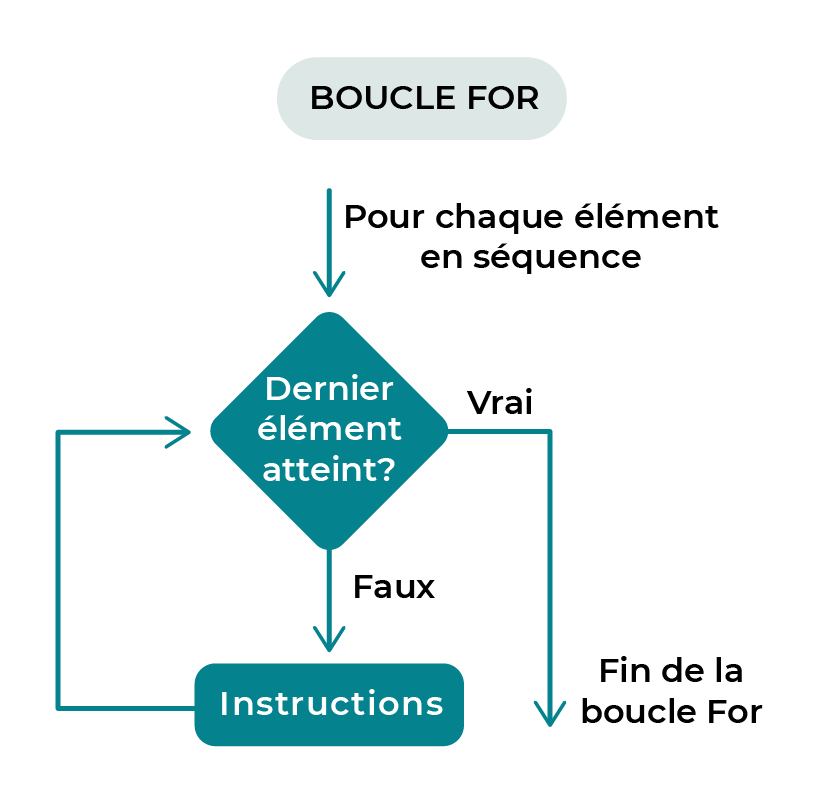
\includegraphics[scale=.3]{Images/boucles/for-loop}
		\caption{Schéma fonctionnel d'une boucle for}
		% Source : https://openclassrooms.com/fr/courses/7168871-apprenez-les-bases-du-langage-python/7296286-repetez-des-taches-facilement-a-l-aide-de-boucles
		%TODO : make smtg similar in latex 
\end{center}\end{figure}

\begin{myexample}
	L'exemple suivant permet d'afficher la liste des collèges de Genève. Pour chaque élément de la boucle, le programme va exécuter l'instruction print en attribuant à la variable |college| la valeur suivante du tableau.
\end{myexample}
%
%\lstset{caption={Boucle for - parcours tableau}}
%\begin{lstlisting}
%	collegesGe = [ "Alice Rivaz" ,  "Calvin" ,  "Claparède",  "de Candolle", 
%	"de Saussure",  "Rousseau",  "Sismondi",  "Voltaire", 
%	"André-Chavanne", "Emilie Gourd",  "Madame de Stael"]
%	
%	print("Voici la liste des collèges de Genève :")
%	for college in collegesGe:
%	print("Collège", college)
%\end{lstlisting}

\begin{myremarque}
	Dans les cas où l'on veut exécuter un bloc d'instructions un nombre précis de fois, la fonction |range(begin,end)| permet de générer un tableau de |begin| à |end-1| qui peut ensuite être utilisé avec une boucle |for|. L'exemple~\ref{ex:counter} peut ainsi être écrit : 
	
\end{myremarque}

\lstset{caption={Boucle for - compteur trivial}}
\begin{lstlisting}[numbers=none]
	maxCompteur = 10
	for compteur in range(maxCompteur+1):
	print(compteur)
\end{lstlisting}

%
%
%%TODO introduce break, continue, else ?
%
